\documentclass[11pt]{article}
\usepackage{amsmath,amssymb,amsfonts,amsthm}
\newcommand{\numpy}{{\tt numpy}}    % tt font for numpy
\usepackage{graphicx}

\topmargin -.5in
\textheight 9in
\oddsidemargin -.25in
\evensidemargin -.25in
\textwidth 7in

\pagenumbering{gobble}

\begin{document}

\begin{enumerate}
% ========== Edit your name here

\item[]{\textbf{Problem 3: LP page 37, Exercise 2.3.1}}
\begin{figure}
    \centering
    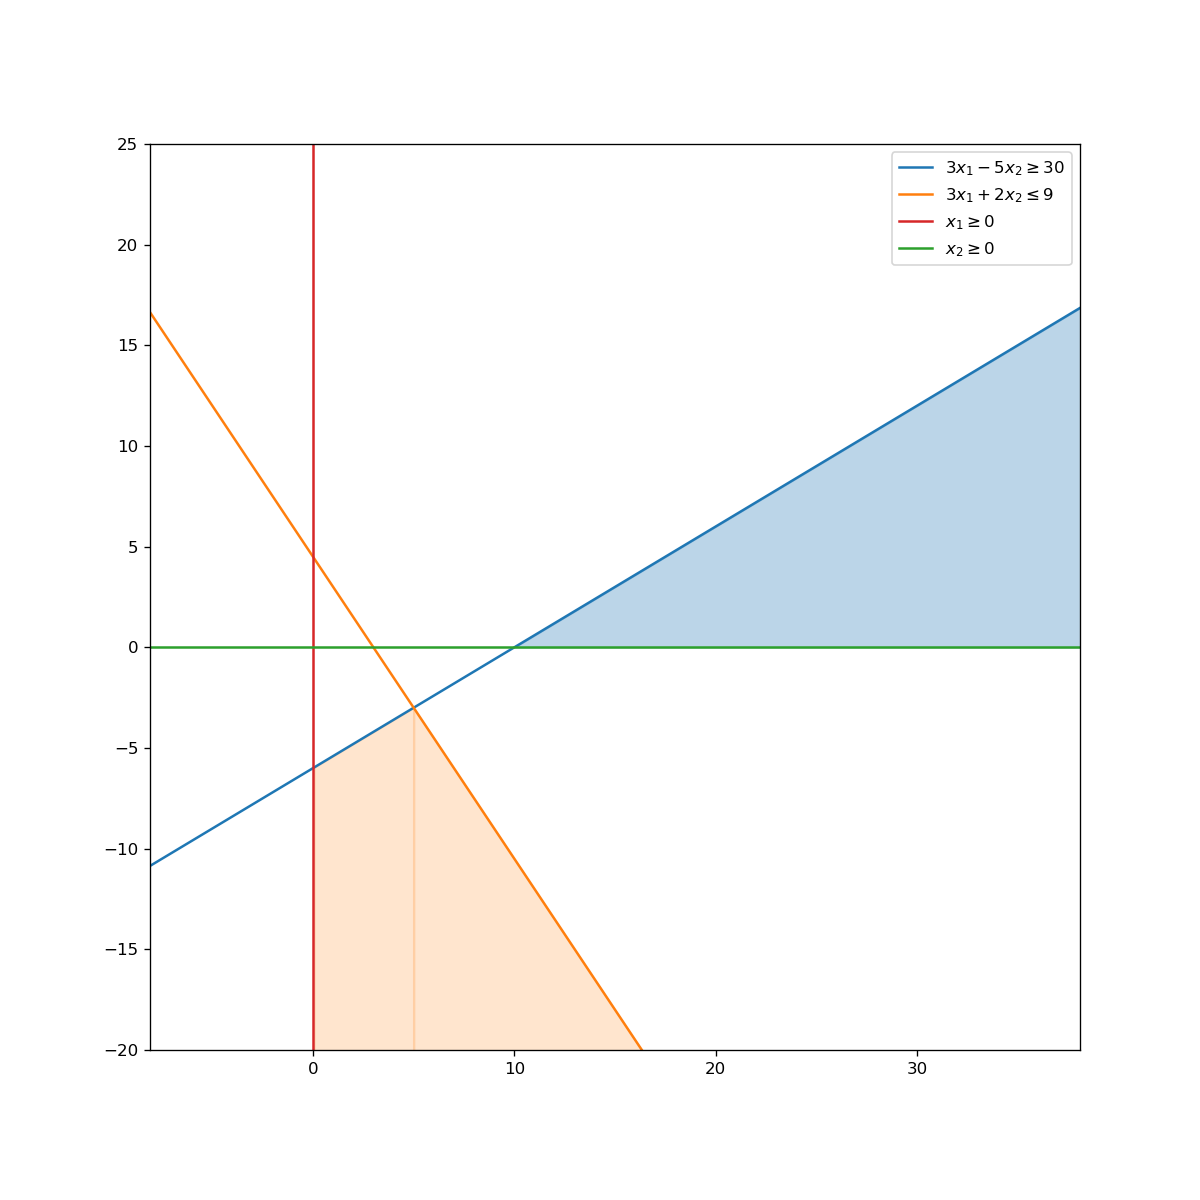
\includegraphics[width=\textwidth]{MSOR411/Homework/4/p3.png}
    \caption{Infeasible regions for Exercise 2.3.1}
    \label{fig:p3}
\end{figure}
\begin{figure}
    \centering
    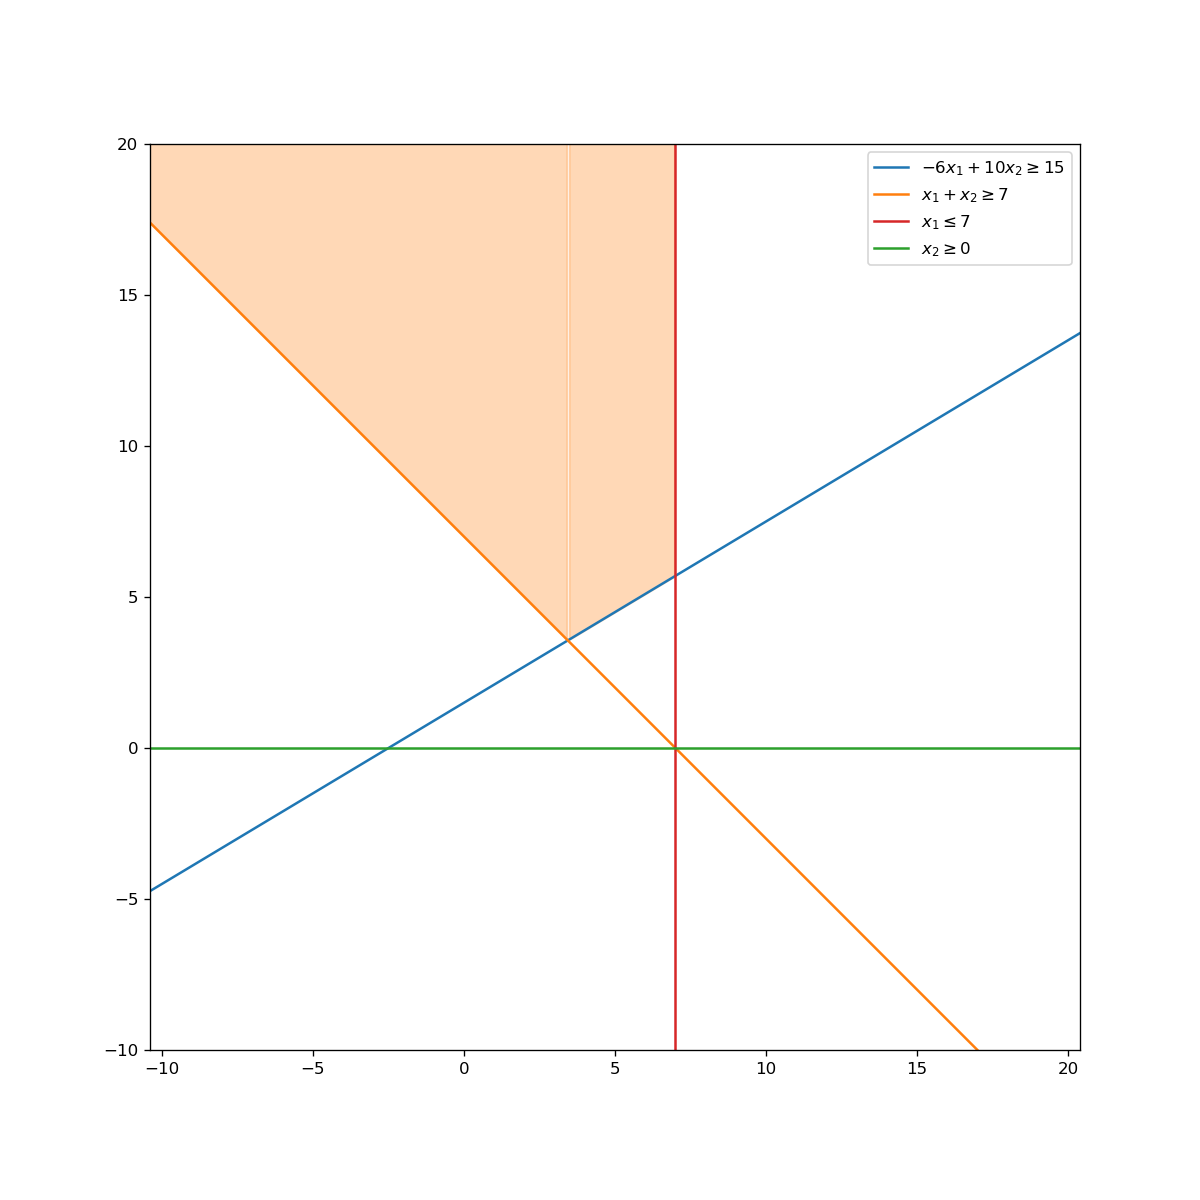
\includegraphics[width=\textwidth]{MSOR411/Homework/4/p4.png}
    \caption{Unbounded region for Exercise 2.4.2} 
    \label{fig:p4}
\end{figure}

For this problem. we have the following constraints:
\begin{align}
    & 3x_1 - 5x_2 \geq 30 \\
    & 3x_1 + 2x_2 \leq 9 \\
    & x_1 \geq 0 \\
    & x_2 \geq 0
\end{align}
However, there exist no points that simultaneously satisfies all four constraints in their defined space. We illustrate this in Figure \ref{fig:p3}. We provide some relaxations on the constraints such that we have two set of constraints: set 1 includes Eq. 1, 3, 4 and set 2 includes Eq. 1, 2, 3. As in Figure \ref{fig:p3}, the two shaded blue and orange regions shows the points in constraint set 1 and 2, respectively. However, there is no intersection between the two shaded region, which means that there is no points in the intersection of constraint set 1 and 2, which is exactly the constraints in the given problem. Thus, this LP problem is infeasible.

\item[]{\textbf{Problem 4: LP page 41, Exercise 2.4.2}}

As shown in Figure \ref{fig:p4}, it is easy to see that the intersection of all constraints of this LP problem is unbounded, as indicated by the shaded orange region. 

\end{enumerate}
\end{document}